\documentclass[12pt,a4paper,UTF8]{ctexart}




%设置页边距
\usepackage{geometry}
\geometry{left=2.5cm,right=2.5cm,top=2.5cm,bottom=2.5cm}
\usepackage{wrapfig}


%需要用到的扩展包

\usepackage{xeCJK,amsmath,paralist,enumerate,booktabs,multirow,graphicx,float,subfig,setspace,listings,lastpage,hyperref}
\usepackage{fancyhdr}




%设置页眉页脚以及页码
\pagestyle{fancy}
\rhead{分光仪的使用}
\lhead{大学基础物理实验报告}
\cfoot{Page\thepage/\pageref{LastPage}}
\rfoot{\today}




%报告中用到的图片存放在这个tex文件所在目录中的figures子目录中
\graphicspath{{figures/}}









%报告开始
\begin{document}
	
	
	
	
	%设置课程标题
	\begin{center}
		\heiti\LARGE{《大学基础物理实验》课程实验报告}
	\end{center}
	
	
	
	
	%设置实验人信息以及实验时间表格
	
	
	\begin{center}
		\begin{tabular}{lcr}
			
			{\songti 姓名及学号:2211082蒋丰毅}  \quad 专业:工科试验班 \quad 年级:22级 \quad 座号:10\\
			{\songti  学院:软件学院 \quad 实验组别:C组\quad 实验时间:2023年4月21日~星期五~上午}\\
			
			
		\end{tabular}
	\end{center}
	\vspace{-0.2cm}
	{\noindent}	 \rule[-10pt]{16cm}{0.05em}\\
	
	\vspace{-0.4cm}
	
	
	
	
	
	
	%实验题目
	\begin{center}
		\LARGE\textbf{分光仪的使用}
	\end{center}
	
	
	\subsection*{[实验目的]}
    \par 1.了解分光仪的结构和原理。
    \par 2.掌握分光仪的调节和使用方法。
	%实验原理
	\subsection*{[实验器材]}
	

\par
	\begin{figure}[!htbp]
	\centering
	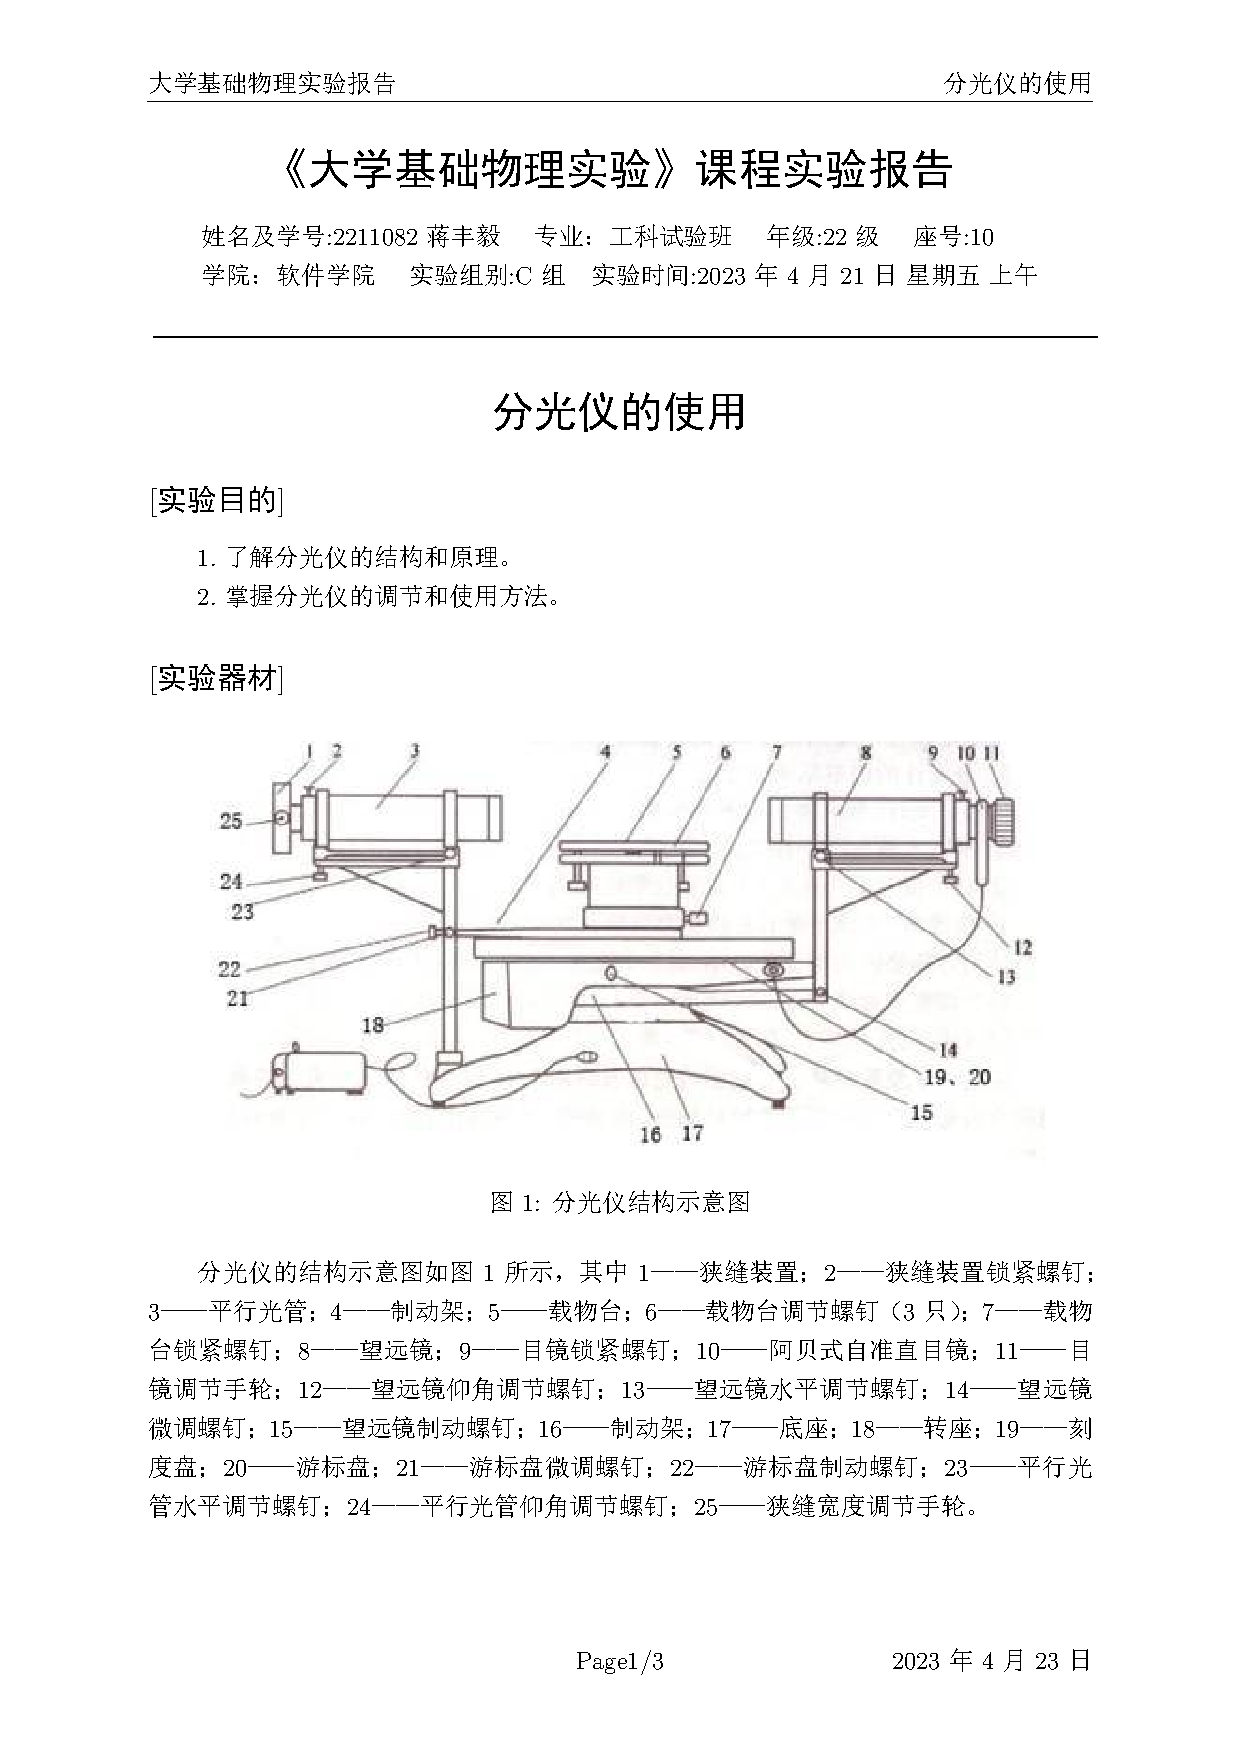
\includegraphics[width=0.9\textwidth]{分光仪.jpg}
	\caption{分光仪结构示意图}
\end{figure}
\par 分光仪的结构示意图如图1所示,其中1——狭缝装置;2——狭缝装置锁紧螺钉;3——平行光管;4——制动架; 5——载物台;6——载物台调节螺钉(3只);7——载物台锁紧螺钉;8——望远镜;9——目镜锁紧螺钉;10——阿贝式自准直目镜;11——目镜调节手轮;12——望远镜仰角调节螺钉;13——望远镜水平调节螺钉;14——望远镜微调螺钉;15——望远镜制动螺钉;16——制动架;17——底座;18——转座;19——刻度盘;20——游标盘;21——游标盘微调螺钉;22——游标盘制动螺钉;23——平行光管水平调节螺钉;24——平行光管仰角调节螺钉;25——狭缝宽度调节手轮。
\clearpage

\begin{figure}[!htbp]
	\centering
	\includegraphics[width=0.9\textwidth]{望远镜.jpg}
	\caption{望远镜结构示意图}
\end{figure}
\par 1.底座——中心有一竖轴,望远镜和读数圆盘可绕该轴转动,该轴也称为仪器的公共轴或主轴。

\par 2.平行光管——是产生平行光的装置,管的一端装有会聚透镜,另一端是带有狭缝的圆筒,狭缝宽度可以根据需要调节。

\par 3.望远镜——观测用,由物镜和目镜系统组成,为了调节和测量,物镜和目镜之间还装有分划板,它们分别置于内管、外管和中管内,三个管彼此可以相互移动,也可以用螺钉固定。参看图2,目镜在内管中,分划板在中管中,分划板下方紧贴一块45°的全反射棱镜,棱镜与分划板的粘贴部分涂成黑色,仅留一个绿色的小十字窗口。光线从小棱镜的另一直角边入射,从45°反射面反射到分划板上,透光部分便形成一个在分划板上的明亮的十字窗。

\par 4.载物台——放平面镜、棱镜等光学元件用。台面下三个螺钉可调节台面的倾斜度。

\par 5.读数圆盘——是读数装置。由可绕仪器公共主轴转动的刻度盘和游标盘组成。度盘上有720等分刻线,格值为30′。有两个角游标。这是因为读数时,要读出两个游标处的读数值,然后取平均值,这样可以消除偏心误差。
\subsection*{[实验原理]}
\par 打开所有的灯光,调节设备使得有成像。
\subsubsection*{粗调}
\par 从正面和上面观察装置,使得望远镜和平行光管刚好在同一条直线上。
\subsubsection*{利用自准法将望远镜调焦于无穷远处}
\par 载物台上放有一块半透半反镜,会将叉丝像反射。调节平面反射镜和望远镜的俯仰使得从望远镜中能看到反射回来的叉丝像,此时对望远镜进行调焦,使得返回的叉丝像变得清晰,并且与叉丝之间没有视差的时候,叉丝与叉丝像都位于望远镜物镜的焦平面上。
\subsubsection*{用各半调节法使望远镜的光轴与仪器转轴垂直}
\par 借助反射镜来进行:
\begin{figure}[!htbp]
	\centering
	\includegraphics[width=0.8\textwidth]{各半调节法}
	\caption{各半调节法示意图}
\end{figure}
\par 完成第二步调节后,进一步调节反射镜和望远镜的俯仰将叉丝像和叉丝重合。这时不能说明望远镜的光轴和仪器的中心转轴相互垂直。将平面镜旋转一百八十度,有可能出现在望远镜里看不到反射回来的叉丝像的现象,这时应当,这时应当调节俯仰,使得叉丝像在旋转前后都在望远镜内。再次将平面反射镜一面反射的叉丝像与叉丝调节重合,将平面镜翻转180度之后,发现叉丝像跟叉丝调节偏差了$d$的距离,调节望远镜的俯仰使得反射叉丝像向叉丝移动$\frac{d}{2}$的距离。在此之后,再调节反射镜的俯仰,使反射叉丝像和叉丝重合。事实上需要重复几次,因为目测很难确定$\frac{d}{2}$的位置。
\subsubsection*{使得平行光管射出平行光,调节其光轴和仪器垂直}
\par 调节狭缝与平行光管物镜之间的距离,直至能从望远镜中观察到边缘清晰,而且与叉丝之间无视差的狭缝像,再次调节平行光管的俯仰,使得狭缝上下对称与望远镜视场的中心的水平叉丝。

\begin{center}
	至此调节完毕
\end{center}
\subsection*{[问题和反思]}
\par 1.本实验调节旋钮较多,实验过程中由于不知道旋钮的作用耽误了很多时间。
\par 2.在使用对半调节法时候,最好的办法其实是目测是否垂直,这样可以省下大量调节旋转前后反射的叉丝像都在望远镜内的时间。
\par 3.一定要一步一步来!前几步一定要确定调整好了,后面就不能在移动之前调整好的东西了,这一步让我损失了大量时间。

\end{document}
